\documentclass{beamer}
\usepackage{listings}

\usetheme[alternativetitlepage=normal]{Rub}
\setbeamercovered{invisible} 
\usepackage{graphicx} % Required for inserting images


\title{Z3 - Tutorial}
\author{Timo Lobitz}
\date{July 2024}

\begin{document}

\maketitle
\begin{frame}{Introduction}
\begin{enumerate}
    \item Smartphone company OnePluZ3 is about to launch their new flagship phone
    \item You are facing several issues that need to be solved ASAP
\end{enumerate}
    
\end{frame}
\begin{frame}{Problem 1 - What to produce?}
\begin{itemize}
    \item You can produce 3 different items
    \begin{itemize}
        \item Phone cases, chargers, and smartphones
    \end{itemize}
    \item Each take different amounts of resources to produce and generate a different amount of profit
    \item You have limited labor hours, machine hours and material available
\end{itemize}
    
\end{frame}

\begin{frame}{Problem 1 - What to produce?}
Resources available:
\begin{itemize}
    \item 500 labor hours
    \item 800 machine hours
    \item 600 units of material
\end{itemize}

\begin{table}
    \centering
    \begin{tabular}{cccccc}
        Name &  Profit & Labor Hours & Machine Time & Raw Materials \\
        Phone Case &  10 & 3 & 3 & 4\\
        Phone Charger & 30  & 5  & 3 &2 \\
        Smartphone & 50  & 4 & 5 & 6\\
    \end{tabular}
    \label{tab:resource_cost}
\end{table}
    
\end{frame}

\begin{frame}{Problem 1 - Formalization}
This can be expressed as a linear programming problem.  
\begin{align}
\max f(x) = 10 * A + 30 * B + 50 * C \\
\text{with contraints}\\
3*A + 5*B+ 4*C <= 500 \\
3*A + 3*B + 5*C <= 800 \\
4*A + 2*B + 6*C <= 600 \\
A>=0 \\
B>=0 \\
C>=0
\end{align}
\end{frame}

\begin{frame}{Problem 2 - Dependency Chaos}
	As part of the production line, you need to manage different parts and chips that are used in different devices.
	\begin{figure}
		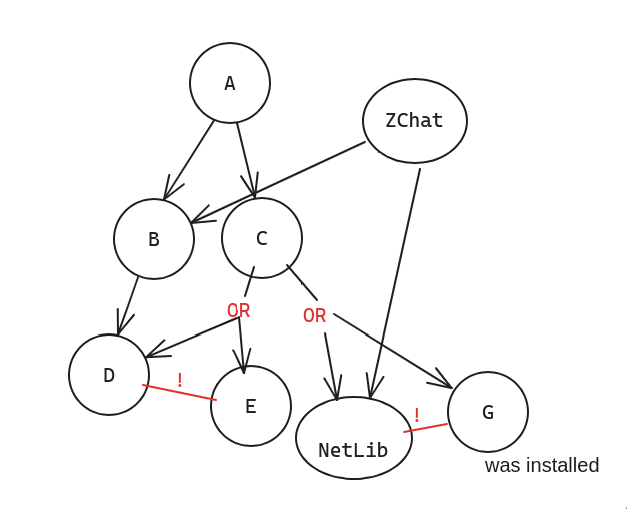
\includegraphics[scale=0.25]{../Images/deps.png}
	\end{figure}
\end{frame}

\begin{frame}{Problem 2 - Formalization}
	\begin{itemize}
		\item Each part is represented by a boolean variable
		\begin{itemize}
		\item True if in production
		\item False if not in production
		\end{itemize}
		\item A depends on B : $A \implies B$
		\item A conflicts with B : $\neg A \lor \neg B$
	\end{itemize}
\end{frame}



\begin{frame}{Problem 3 - Code Verification}
The day 1 patch is currently in code review. You notice a strange function written by a coworker.
\lstinputlisting[language=c]{magic.c}
\end{frame}


% Z3 Introduction
\begin{frame}{Z3}
\begin{columns}
\begin{column}{0.5\textwidth}
	\begin{itemize}
		\item SMT solver
		\item open-source
		\item from Microsoft Research
	\end{itemize}
\end{column}
\begin{column}{0.5\textwidth}
	\begin{figure}
		
\includegraphics[scale=0.3]{../Images/z3logo.png}
	\end{figure}
\end{column}

\end{columns}

\end{frame}

\begin{frame}{Z3 - Usage}
	
	
\begin{columns}
	\begin{column}{0.4\textwidth}
		4 Step pattern:
		\begin{enumerate}
			\item Create Solver
			\item Define variables
			\item Add constraints
			\item Check
		\end{enumerate}
	\end{column}
	\begin{column}{0.6\textwidth}
		\pause
		\lstinputlisting[language=python]{usage.py}
		
	\end{column}
	
\end{columns}
\end{frame}


\begin{frame}{Variables}
	
\begin{columns}
	\begin{column}{0.4\textwidth}
			\lstinputlisting[language=python]{variables.py}
	\end{column}
	\begin{column}{0.6\textwidth}
			\lstinputlisting[language=python]{variables2.py}
		
	\end{column}
	
\end{columns}


\end{frame}

\begin{frame}{Arrays}
	Arrays in Z3 map from one datatype to another. They support Store and Select operations.
	\lstinputlisting[language=python]{arrays.py}
	
\end{frame}

\begin{frame}{Custom Datatypes - Enum}
	\lstinputlisting[language=python]{enum.py}
\end{frame}


\begin{frame}{Custom Datatypes - List}
	\lstinputlisting[language=python]{list.py}
\end{frame}

\end{document}
